
%\documentclass[english]{ipsj}
%\documentclass[english,preprint]{ipsj}
\documentclass[english,preprint,JIP]{ipsj}


%% 追加
\usepackage{bm}
\usepackage{url}
\usepackage{color}
% \usepackage{ulem}
%% ここまで


\usepackage{graphicx}
\usepackage{latexsym}

\def\Underline{\setbox0\hbox\bgroup\let\\\endUnderline}
\def\endUnderline{\vphantom{y}\egroup\smash{\underline{\box0}}\\}
\def\|{\verb|}


\setcounter{volume}{26}% vol25=2017
\setcounter{number}{1}%
\setcounter{page}{1}


\received{2016}{3}{4}
%\rereceived{2011}{10}{1}   % optional
%\rerereceived{2011}{10}{31} % optional
\accepted{2016}{8}{1}



\usepackage[varg]{txfonts}%%!!
\makeatletter%
\input{ot1txtt.fd}
\makeatother%

\begin{document}

\title{User Identification Method based on Head Shape\\
using Pressure Sensors embedded in a Helmet}

\affiliate{Rits}{Ritsumeikan University, Kusatsu, Shiga 525--8577, Japan}
\affiliate{JST}{PRESTO, Japan Science and Technology Agency, Kawaguchi, Saitama 332–0012, Japan}

\author{Atsuhiro Fujii}{Rits}[atsuhiro.fujii@iis.ise.ritsumei.ac.jp]
\author{Kazuya Murao}{Rits,JST}[murao@cs.ritsumei.ac.jp]


\begin{abstract}
Various types of helmets exist, including industrial protective helmets, motorcycle helmets, sports helmets, and military/police helmets. By identifying individuals wearing a helmet, their name, affiliation, and qualification can be presented on a display mounted on the helmet, and sensor data collected through the helmet, such as acceleration, video, and eye-tracking data, can be labeled with the user's ID. In this paper, we propose a user identification method based on head shape using a helmet equipped with 32 pressure sensors. Our method has two functions: user identification and authentication. \textcolor{red}{User identification is based on the assumption that a single helmet is shared by multiple individuals. The goal of this method is to identify which of the registered people is the person wearing the helmet. SVM is trained by head data from the users we want to identify. Then, the input data obtained when the helmet is worn is classified and the user is identified. User authentication determines whether the individual wearing the helmet is the individual with the ID when the ID is provided to the system. The head data of the user to be authenticated is collected several times. Then, the system calculates the Mahalanobis distance between the input data obtained while wearing the helmet and the pre-collected data set. A user is authenticated if the distance is less than the threshold and is rejected if it is greater than the threshold. We implemented the prototype device and evaluated our proposed method. In the evaluation, we obtained sensor values for 2 seconds 20 times from nine subjects as head shape data. The accuracy was evaluated using 5-fold cross-validation, and we achieved 100\% accuracy with five sensors and 92\% with two sensors for user identification and an average equal error rate of 0.076 with 32 sensors for user authentication.}

% Various types of helmets exist, including industrial protective helmets, motorcycle helmets, sports helmets, and military/police helmets. By identifying individuals wearing a helmet, their name, affiliation, and qualification can be presented on a display mounted on the helmet, and sensor data collected through the helmet, such as acceleration, video, and eye-tracking data, can be labeled with the user's ID. In this paper, we propose a user identification method based on head shape using a helmet equipped with 32 pressure sensors. Our method has two functions: user identification and authentication. Identification aims to classify a user as a registered user, while authentication aims to accept users who are registered in the system and reject unknown users. We implemented a prototype helmet device and collected data from nine subjects, resulting in 100\% accuracy for user identification and an average equal error rate of 0.076 for user authentication.
\end{abstract}

\begin{keyword}
User identification, pressure sensor, helmet, head shape
\end{keyword}

\maketitle

%1
\section{Introduction}
\label{sec:introduction}
There are various types of helmets, such as industrial protective helmets, motorcycle and bicycle helmets, sports helmets (for American football, baseball, ice hockey, etc.), and military/police helmets. These are all worn to protect the head in the event of an accident\cite{helmet}. From a safety point of view, it is important that there is no gap between the head and the helmet.\par

Workers in factories and disaster sites must also often wear helmets. Wearing a helmet can allow individuals who do not know each other, such as classroom use is granted without fee provided that copies are not made or distributed short-term workers and vendors, to be identified by displaying their names and work division on their helmets. Helmets can also allow wearers to be identified from a distance or overhead even if their faces cannot be clearly seen. Identifying individuals also serves as a deterrent to trespassers. In addition, displaying qualifications, such as a hazardous materials engineer's license and a heavy machinery license, can help create a safe work environment. In many cases, this information is written directly on the helmet, or an identifiable sticker is attached to the helmet. However, such an analog system makes it possible for trespassers to easily disguise themselves by forging or stealing a sticker. In addition, a worker can put on another worker's helmet without being aware of it, and incorrect information will be displayed. If helmets are shared among workers, they are not marked with identifiable information.\par

In this paper, we propose a method that identifies users based on the shape of their heads by installing pressure sensors inside a helmet. We implemented a prototype helmet with 32 pressure sensors. Our method calculates the similarity between the wearer's data and registered users' data and outputs the user with the most similar data.\par

The prototype helmet has a display to indicate the user's name and credentials based on the identification results; therefore, incorrect information is not displayed on the helmet if a helmet belonging to someone else is used. One advantage of this system is that identification information is automatically displayed on a shared helmet, allowing workers to identify each other. Another advantage of user identification is data annotation. Data collected by sensors attached to the helmet or wearer's body, such as a camera, eye tracker, and accelerometer, can be automatically annotated with the wearer's ID. By attaching a Global Positioning System (GPS) module or antenna to localize the user\cite{disaster_en}, the name and location of a worker can be determined in real time, allowing the foreperson to have a better understanding of the overall situation in the field. Furthermore, from the pressure data between the helmet and the head, it is possible to verify whether the shape of the head matches the helmet, as a zero pressure value signifies that there is a gap between the helmet and head. Another potential use of the proposed helmet is to serve as a key to a room whose access is restricted based on one's position or qualifications.\par

The proposed method has two functions: user identification and authentication. User identification is based on the assumption that a single helmet is shared by multiple individuals. The pressure sensor data of an individual who may wear a helmet are registered in advance, and an individual wearing a helmet is identified as one of the registered persons. Personal identification does not take into account that a non-registered individual may wear the helmet; if a non-registered individual wears the helmet, the identification result will be a registered user who has the most similar data to the wearer. User authentication determines whether the individual wearing the helmet is in fact the individual with the ID when the ID is provided to the system. We assume an environment in which all individuals have their own helmets (as in smartphone authentication). In addition, we assume an environment in which the user ID is entered when using a shared helmet (as in automated teller machine [ATM] authentication). Even if an intruder wears a helmet and enters a stolen ID, he or she can be identified as an intruder (authentication denied) because the head shape differs from that of the individual with the ID. \textcolor{red}{This helps avoid the risk of motorcycle theft. For example, the helmet and the motorcycle are paired in advance, then theft of the motorcycle can be prevented by authenticating the user when riding.}\par

The remainder of this paper is organized as follows. Section \ref{sec:related} introduces related work, Section \ref{sec:method} describes the proposed method, Section \ref{sec:evaluation} evaluates the proposed method, Section \ref{sec:limitation} describes limitation of the proposed method, and Section \ref{sec:conclusion} concludes the paper.



%2
\section{Related Work}
\label{sec:related}
In this section, we introduce research on user identification and head state recognition.


%2.1
\subsection{User Authentication Method}
There are several methods for identifying individuals: password, personal identification number (PIN), and stroke pattern; physical characteristics, such as face, fingerprint, voice print, and iris; and behavioral characteristics, such as handwriting and gait. However, passwords, PINs, and stroke patterns that can be freely set by individuals have a risk of spoofing by shoulder hacking, brute force attacks, and password duplication.\par

For physical characteristics, Chen et al.\cite{face_and_finger} proposed an authentication method using video images of the user's face and fingertips captured from the front and rear cameras of a mobile device. Siddharth et al.\cite{palm_print} proposed an authentication system based on the palm print and palm vein. The system uses visible and infrared light to acquire images of the palm print and palm vein, and authentication is performed by verifying the data against registration data in the database. Sayo et al.\cite{lip_motion} proposed an authentication method based on a camera image that captures the shape of a user's lips (physical characteristic) and the movement of the lips during speech (behavioral characteristic). Another authentication method involving the mouth proposed Kim et al.\cite{teeth_and_voice} combines dental images and voice. Bednarik et al.\cite{eye_movement} proposed an identification system that uses eye movements, such as pupil size and variation, gaze velocity, and the distance of the infrared reflection of the eye. Barros Barbosa et al.\cite{nail_auth} showed that images of the fingernail plate can be used as a transient biometric with a useful life-span of less than 6 months. Using a camera-based approach such as the ones described above, a camera can be mounted on the outside of the helmet, and individuals can be identified by facing the camera before putting on the helmet. However, taking a picture of one's own face with the camera is complication. 
%\textcolor{red}{In addition, taking pictures with a camera has privacy issues.} 
Using the palm print and palm vein method, users would have to hold the camera each time before putting on the helmet. It is also complication. 
%\textcolor{red}{\sout{A camera can be attached to the mouth of the helmet so that the shape and movement of the wearer's lips and teeth can be acquired. However, the space around the mouth inside a full-face helmet is limited, and it is difficult to distinguish the shape and movement around the mouth with a single camera.}} 
In addition, this approach is not practical because helmets are sometimes used in \textcolor{red}{the rain. In the case of authentication methods that use images from a camera, the accuracy may be degraded if the camera lens is covered with water droplets or dust.}\par

\textcolor{red}{Nogueira et al.\cite{finger_CNN} used convolutional neural networks for fingerprint authentication and achieved high classification accuracy. However, fingerprint authentication requires the user to touch the sensor for each authentication. In contrast, our method does not require any specific behavior.}
Schneegass et al.\cite{skull_auth} proposed a biometric user identification method using that the way sound is transmitted through the head differs from person to person. They played white noise from a bone conduction speaker attached to the side of the head, received signals using a microphone, and identified the subjects based on their characteristics. As a result, they achieved 97.0\% accuracy. Dai et al.\cite{speech_auth} proposed SpeakPrint, a human speech authentication scheme for smartphones which is resistant for attacks such as spoofing, based on the user's mouth movements and the voice changes. Jian et al.\cite{voice_auth_GMM} proposed the process of voiceprint recognition with Gaussian mixture model (GMM) which is a kind of probability and statistics model. Zhang et al.\cite{voice_auth_DNN} constructed a voiceprint recognition model using DNN to achieve higher recognition performance. However, the experiment showed that the DNN-based voiceprint recognition system still had a low accuracy rate of rejection of counterfeiters. For this reason, the trust degree and label distance were introduced, and the two-order judgment structure based on DNN-RLIANCE algorithm was proposed. These are studies on authentication methods that use sound. The helmet may be used in noisy environments such as construction sites, so these authentication methods are not suitable.\par

% Nogueira et al.\cite{finger_CNN} used convolutional neural networks for fingerprint authentication and achieved high classification accuracy. However, the limitation of fingerprint authentication is that fingerprints can be easily duplicated from photographs. In contrast, head shape, which is used in this paper, is a physical characteristic that is difficult to replicate due to its three-dimensional shape.\par

With respect to behavioral characteristics, the authors proposed a method that authenticates smartphone users using acceleration sensor data from taking a smartphone out of their pockets\cite{murao_screen_unlock_blind}. Guerra-Casanova et al.\cite{accelerometer_authentification} proposed a method for authenticating users by the gestures of their hands using a mobile device with an embedded accelerometer. For motion-based authentication using accelerometers, it is possible to use the acceleration characteristics of motions before the helmet is put on for authentication by mounting an accelerometer on the helmet. \textcolor{red}{We think that the helmet-wearing motion is not highly reproducible. As for the motion of taking the smartphone out of the pocket, the reproducibility is high because the movement is restricted to some extent. However, the helmet is worn with one hand, two hands, or in a different direction, and there are a variety of actions from picking up the helmet to putting it on. Therefore, it is not practical to collect data from all individuals for various situations.}

% With respect to behavioral characteristics, the authors proposed a method that authenticates smartphone users using acceleration sensor data from taking a smartphone out of their pockets\cite{murao_screen_unlock_blind}. Guerra-Casanova et al.\cite{accelerometer_authentification} proposed a method for authenticating users by the gestures of their hands using a mobile device with an embedded accelerometer. For motion-based authentication using accelerometers, it is possible to use the acceleration characteristics of motions before the helmet is put on for authentication by mounting an accelerometer on the helmet. However, there are various ways of putting on a helmet, such as putting it on in a hurry and taking care not to let the interior of the helmet become wet in the rain. Therefore, it is not practical to collect data from all individuals for various situations.


%2.2
\subsection{User Authentication Method with Pressure Sensors}
Chen et al.\cite{driver_handgrip_1}, \cite{driver_handgrip_2} proposed a user authentication method based on the driver's grasping pattern using a pressure sensor sheet attached to the handlebars of a bicycle. In Reference \cite{driver_handgrip_1}, the authentication decision was made using the features of the grasp data obtained from the pressure sensor sheet. The experimental results obtained in this study show that the mean acceptance rates of 78.15\% and 78.22\% for the trained subjects and the mean rejection rates of 93.92\% and 90.93\% to the un-trained ones are achieved in two trials, respectively. In Reference \cite{driver_handgrip_2}, authentication was performed using time series data of pressure values. The experimental results obtained in this study show that mean acceptance rates of 85.4\% for the trained subjects and mean rejection rates of 82.65\% for the un-trained ones are achieved by the classifier in the two batches of testing. Iso et al.\cite{mobile_grip} proposed a user authentication method by using a pressure sensor array mounted on the side of a mobile phone to identify the grasping state of the phone during use. The authors proposed a user authentication method using pressure sensors mounted on the side and back of a mobile phone, based on a pre-registered gripping method\cite{murao_grip}.\par

These are all researches on authentication methods based on behavioral characteristics such as grasping using a pressure sensor. On the other hand, we use a pressure sensor to obtain physical characteristics for user authentication.


%2.3
% \subsection{Head State Recognition}
% \sout{Toth et al.\cite{facial_expression_headset} focused on facial muscle signals, and six different facial expressions were classified using muscle signals and gyroscope values that were obtained from a low-cost off-the-shelf electroencephalogram (EEG) headset. EEG headsets are generally used to measure brain waves; however, muscle signals are detected locally because the measurement is performed by placing electrodes on the scalp. This method only uses existing EEG devices for the classification of facial expressions, and no additional electromyography sensors are used. Kwon et al.\cite{facial_expression_glasses} designed a glasses-type wearable device to detect a user's emotions based on facial expressions and physiological reactions. The device can capture facial expressions with a built-in camera and detect physiological responses, such as photoplethysmogram signals and electrodermal activity. Fukumoto et al.\cite{fukumoto} designed a smile-based life-logging system that focuses on smile and laughter to index interesting or enjoyable events on recorded video. They used photointerrupters, and smile/laughter was detected separately by threshold-based clustering. The evaluation results demonstrated a 73–94\% accuracy in detecting smile/laughter during actual use of the system.\par

% These studies all use dynamic information, such as facial expressions and physical movements in the facial area. In contrast, our study uses static features of head shape.\par

% In other research, Kouno et al.\cite{head_top_camera} proposed an image-based person identification system using depth images from an overhead camera. By using depth information, this system captures the precise location of the individual, and four features are extracted from the images: body height, body dimensions, body size, and a depth histogram. The identification accuracy was 94.4\% and 91.4\% while standing in front of a door and touching a doorknob, respectively.\par

% In this paper, we propose a method for identifying individuals by acquiring their head shape with pressure sensors while they wear a helmet. Our method does not require individuals to perform special behaviors or remain stationary for identification. With a wearable approach, our method can be used at any place and time. To breach the system, the exact three-dimensional shape of a person's head is required, which is difficult to replicate.}



%3
\section{Proposed Method}
\label{sec:method}
In this section, we present the details of the proposed method.


%3.1
\subsection{Overview}
The proposed method assumes that a user wears a helmet equipped with pressure sensors. It then acquires the shape of the wearer's head and determines whether the wearer is a registered user. The proposed method has two functions: user identification and authentication.
\begin{itemize}
    \item {\bf User identification} assumes that a single helmet is shared by multiple people and that no other information, such as the ID, is provided to the system; the user simply puts on the helmet. Users' pressure sensor data are registered in advance, and a user who puts on a helmet is identified as one of the registered users. User identification does not consider that a non-registered person may put on the helmet. If a non-registered person puts on the device, the identification result will be an individual with the closest data among the registered users.

    \item {\bf User authentication} determines whether the individual wearing the helmet is the correct individual when his/her ID or username is provided. We assume two cases in which authentication is used: (i) each individual has his/her own helmet and only the individual's pressure sensor data have been registered (single user; username is preset on device, as in smartphone authentication); and (ii) a helmet is shared among multiple users, and a username is entered when putting on the helmet (multiple users; usernames are input manually, as in ATM authentication). The pressure sensor data are registered in advance, and a user who puts on the helmet is accepted or rejected by calculating the similarity between the input data and the data corresponding to the ID. Even if the ID is leaked, an intruder can be rejected if his/her head shape differs from the data corresponding to the ID.
\end{itemize}

The flow of our system is illustrated in \figref{fig:system}. A total of 32 pressure sensors are attached to the inner side of the helmet to acquire data, producing one-dimensional 32-channel pressure data. Pressure data of individuals who are expected to wear helmets are registered in the system in advance and are called training data in this paper. In user identification, the proposed system uses a support vector machine (SVM) to build a recognition model from the feature values extracted from the training data and outputs the identification results from the features of the input data of an unknown registrant. In user authentication, the system calculates the Mahalanobis distance between the training and input data of the user, including non-registrants, and authenticates the user if the distance is less than the threshold; otherwise, the user is rejected.

\begin{figure}[!t]
  \centering
    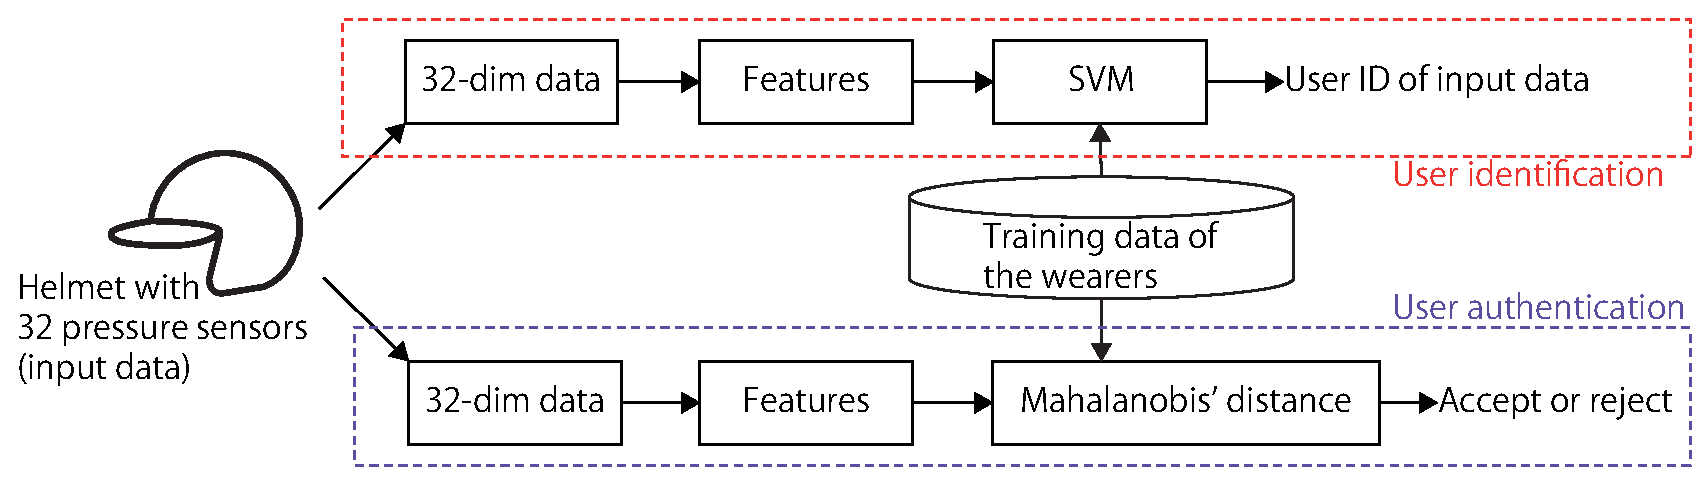
\includegraphics[width=1\linewidth]{figure/system.eps}
  \caption{Process of user identification and authentication.}
  \label{fig:system}
\end{figure}



%3.2
\subsection{Hardware}
We developed a helmet equipped with 32 pressure sensors. \figref{fig:device} presents the configuration of the device, and \figref{fig:met_over} provides an image of the device. The head of the user must be in close contact with the sensors to obtain the correct pressure values; therefore, we used a commercially available full-face helmet ($\approx$ 4,000 JPY). The pressure sensors were FSR402 ($\approx$ 500 JPY) and FSR402 Short Tail ($\approx$ 550 JPY) manufactured by Interlink Electronics, Inc. The Arduino MEGA2560 R3 ($\approx$ 6,000 JPY) was used as a microcomputer. Because the helmets was difficult to attach and remove the interior, we removed the interior of the top of the helmet and installed a thick urethane sponge, as illustrated in \figref{fig:met_in}. The urethane sponge was cut and a pressure sensor was inserted into the cut line, as illustrated in \figref{fig:sensor}.\par

Four pressure sensors were placed at the top of the head, 16 sensors were placed around the top of the head, six sensors were placed at the back of the head, and six sensors were placed at the cheek pads on both sides. A total of 32 sensors were installed at the points, as displayed in \figref{fig:position}. The wiring for the pressure sensors passed through a hole drilled at the top of the helmet and was then connected to a 5V power supply port, GND, and analog input port, which was on the Arduino MEGA2560 R3 via a printed circuit board (PCB) with a 10K$\Omega$ resistor that was mounted outside the helmet. The PCB and a display to show ID attached to the exterior of the helmet are illustrated in \figref{fig:print} and \figref{fig:lcd}. They were bolted to both of the cheek area using a threaded hole drilled to secure the helmet shield, and was fixed and removable.\par

\textcolor{red}{The size of the helmet is shown in \figref{fig:size}. The height, width, and depth of the helmet are 260 mm, 213 mm, and 282 mm, respectively, and the weight including a PCB and a LCD display is 1456 g.}

\begin{figure}[!t]
  \begin{center}
    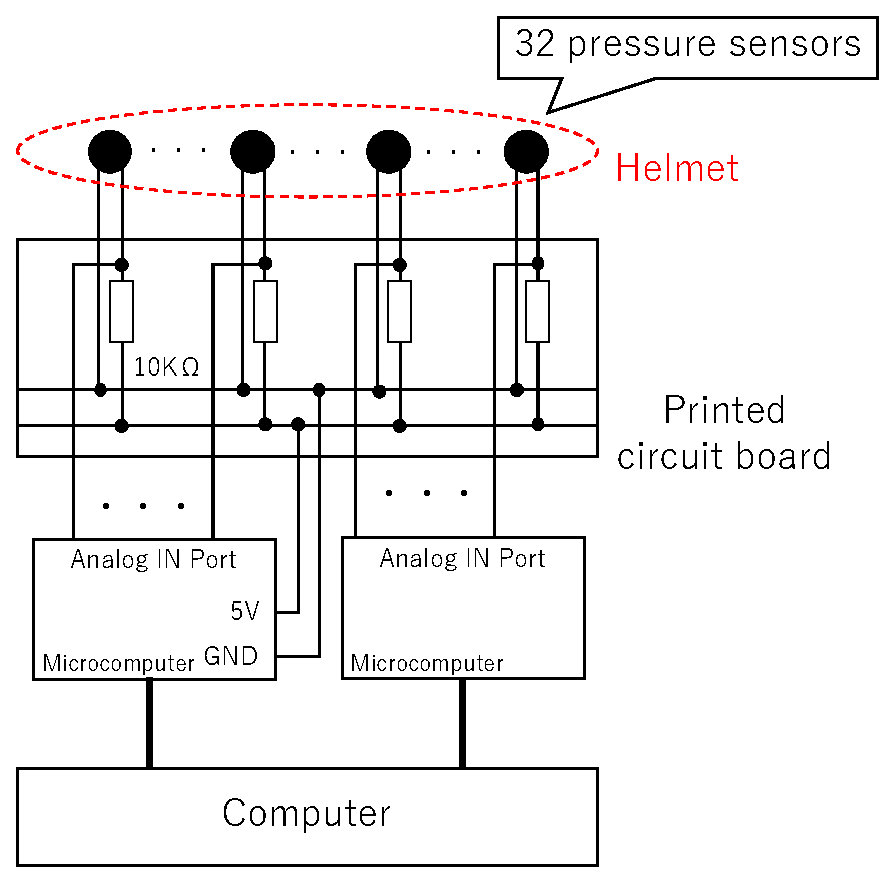
\includegraphics[width=0.6\linewidth]{figure/device.eps}
  \end{center}
  \caption{Structure of device.}
  \label{fig:device}
\end{figure}

\begin{figure}[!t]
  \centering
    \includegraphics[width=0.9\linewidth]{figure/met_over.eps}
  \caption{\textcolor{red}{Appearance of the prototype device.}}
  \label{fig:met_over}
\end{figure}

\begin{figure}[!t]
\begin{minipage}{0.48\hsize}
\begin{center}
        \includegraphics[width=1\linewidth]{figure/met_in.eps}
  \end{center}
  \caption{\textcolor{red}{Interior of}\\\textcolor{red}{the prototype device.}}
  \label{fig:met_in}
  \end{minipage}
\begin{minipage}{0.48\hsize}
\begin{center}
        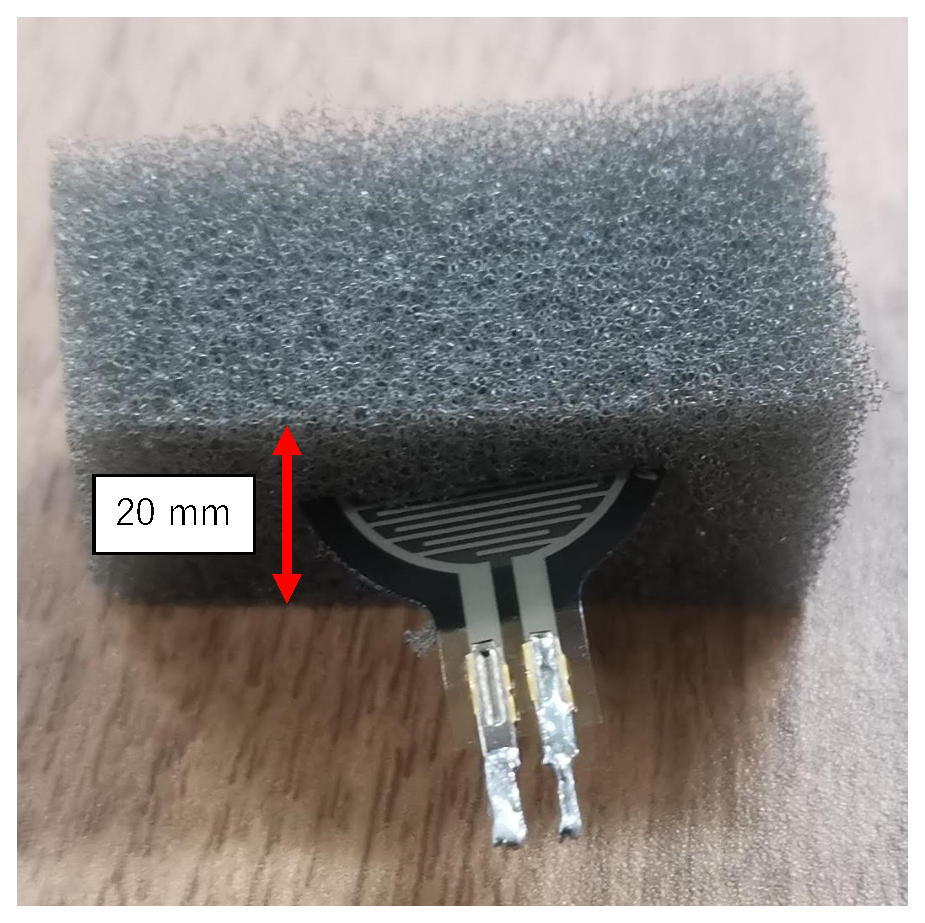
\includegraphics[width=1\linewidth]{figure/sensor.eps}
        \end{center}
  \caption{Pressure sensor mounted in\\the helmet using urethane\\sponge.}
  \label{fig:sensor}
  \end{minipage}
\end{figure}

\begin{figure}[!t]
  \begin{center}
    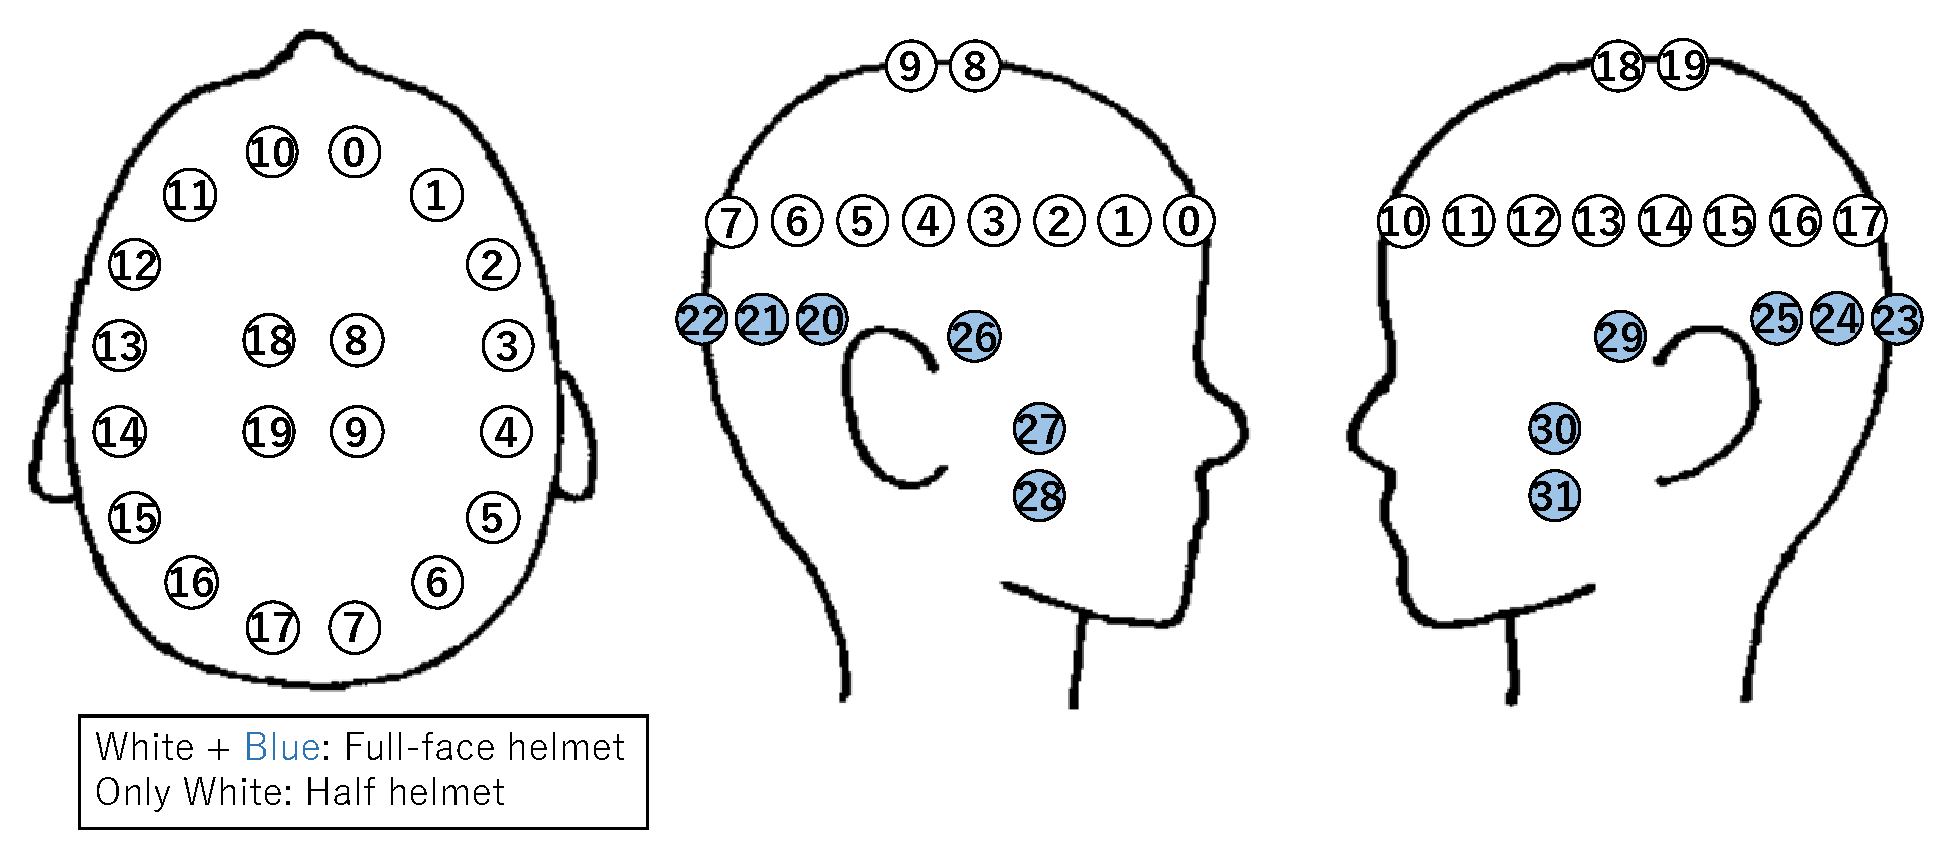
\includegraphics[width=1\linewidth]{figure/position.eps}
  \end{center}
  \caption{Position of pressure sensors.}
  \label{fig:position}
\end{figure}

\begin{figure}[!t]
\begin{minipage}{0.48\hsize}
  \begin{center}
    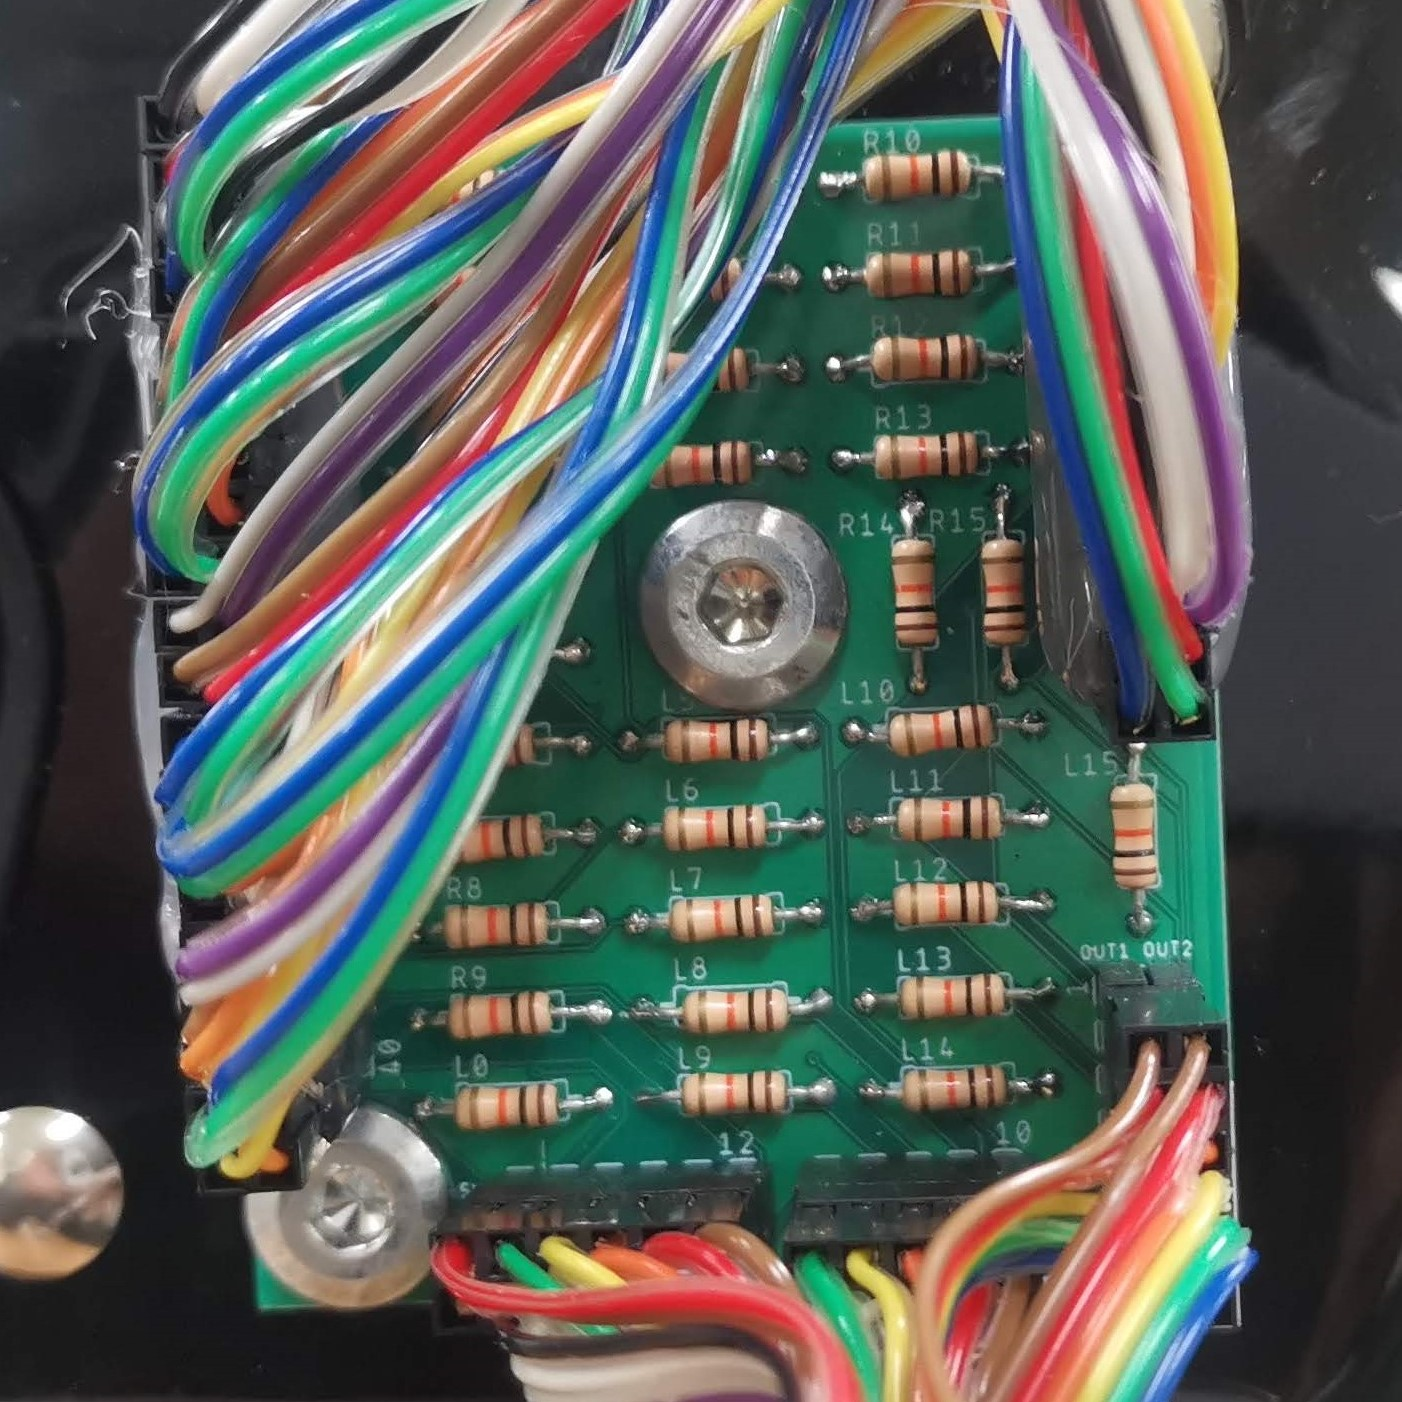
\includegraphics[width=1\linewidth]{figure/print.eps}
  \end{center}
  \caption{Printed circuit board\\connected to 32 pressure\\sensors.}
  \label{fig:print}
  \end{minipage}
\begin{minipage}{0.48\hsize}
  \begin{center}
    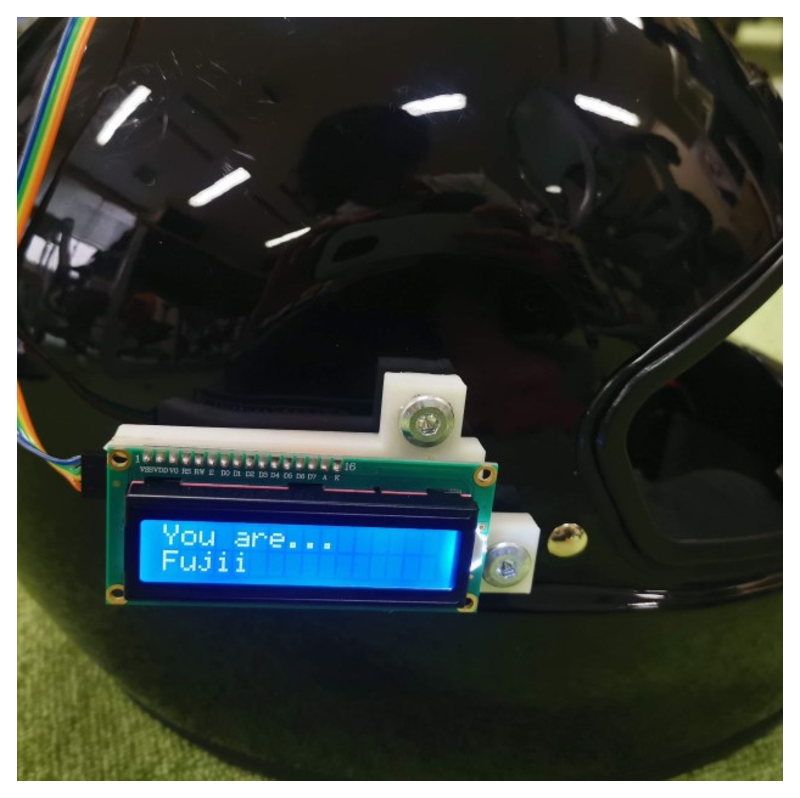
\includegraphics[width=1\linewidth]{figure/lcd.eps}
  \end{center}
  \caption{LCD display to show name.\\~\\~}
  \label{fig:lcd}
  \end{minipage}
\end{figure}

\begin{figure}[!t]
  \begin{center}
    \includegraphics[width=0.9\linewidth]{figure/size.eps}
  \end{center}
  \caption{\textcolor{red}{Size of the prototype device.}}
  \label{fig:size}
\end{figure}



%3.3
\subsection{User Identification Method}


%3.3.1
\subsubsection{Preprocessing.}
Data acquisition begins when a user puts on the helmet. Data from 32 pressure sensors $\bm{p}(t)=[p_1(t),\cdots,p_{32}(t)]$ are acquired at time $t$. The voltage values of all pressure sensors are almost 5V when the helmet is not worn, then sum of the data show $\sum_{i=1}^{32}p_i(t)\approx160[V]$. When the helmet is worn, $p_i(t)$ decreases, and the system segments the data over a 2-s window starting from $t=T_s$ after the values are stabilized. Time $t=T_s$ is the time at which the change of the sum of 32 dimensions per sample is less than 2V for 11 consecutive samples ($\approx$11/30 second as the sampling rate is approximately 30 Hz) after the sum of 32 dimensions is less than 155V, i.e. $\sum_{i=1}^{32}|p_i(t)-p_i(t-1)|<2[V]~(i=T_s,\cdots,T_s-10)$. The average value over the window $x_i(t)=\frac{1}{N}\sum_{t=T_S}^{T_S+N-1}p_i(t)$ for sensor channel $i$ ($i=1,\cdots,32)$ is calculated, where $N$ is the number of samples in the window. We then obtain a 32-dimensional vector $\bm{x}(t)=[x_{1}(t),\dots,p_{32}(t)]$ as a feature. Once the data is segmented, the preprocessing is suspended until $\sum_{i=1}^{32}p_i(t)>159$[V] is met.


%3.3.2
\subsubsection{Identification.}
Given training data $[\bm{x}_m,y_m]$ $(m=1,\dots, M)$ from users who are expected to use the helmet by wearing the helmet a total of $M$ times in advance, the SVM is trained with the training data, where $y_m$ is the registrant label, such as the registrant's name and number. The input data $\bm{x}_{test}$ collected by the user to be identified are fed into the SVM and the classification result $\hat{y}_{test}$ is obtained.


%3.4
\subsection{User Authentication Method}


%3.4.1
\subsubsection{Preprocessing.}
In user authentication, data from 32 pressure sensor data $\bm{p}(t)=[p_1(t),\cdots,p_{32}(t)]$ and the average $\bm{x}(t)=[x_{1}(t),\dots,p_{32}(t)]$ are obtained as a feature in the same manner as for user identification.


%3.4.2
\subsubsection{Similarity calculation.}
In user authentication, there are two cases for using training data: data of a single user are used and data of multiple users are used. For single-user data, data of only a single user (e.g., owner of the helmet) are registered or data of multiple users are registered; however, the data of only one of the users whose ID is provided are used. For multiple-user data, data of multiple users who are expected to use the helmet are used. With training data $[\bm{x}_m,y_m]$ $(m=1,\dots, M)$ obtained from user(s) wearing the helmet $M$ times in advance, the proposed method calculates the Mahalanobis distance, where $y_m$ is the registrant label, such as the registrant's name and number.\par

The Mahalanobis distance is a method for calculating the distance between multiple variables, and can be normalized considering the distribution of the data. The mean vector $\bm{\mu}$ and the variance-covariance matrix $\bm{\Sigma}$ of the training data are calculated by (\ref{eqn:mu}) and (\ref{eqn:sigma}).
\begin{eqnarray}
\label{eqn:mu}
  \bm{\mu} &=& \frac{1}{M}\sum_{m=1}^{M}\bm{x}_m \\
\label{eqn:sigma}
  \Sigma_{i,j} &=& \frac{1}{M}\sum_{m=1}^{M}(\bm{x}_i-\bm{\mu})(\bm{x}_j-\bm{\mu})^T
\end{eqnarray}
 
The Mahalanobis distance between the training data $\bm{x}_m$ $(m=1,\dots, M)$ and input data $\bm{x}_{test}$ can be calculated by (\ref{eqn:mahalanobis}).
\begin{eqnarray}
\label{eqn:mahalanobis}
  d(\bm{x},\bm{x}_m) = \sqrt{(\bm{x}-\bm{x}_m)^{T}\bm{\Sigma}^{-1}(\bm{x}-\bm{x}_m)}
\end{eqnarray}
If the input data are collected from a pre-registered user, the input data $\bm{x}_{input}$ follow the probability distribution of the variance-covariance matrix $\bm{\Sigma}$.


%3.4.3
\subsubsection{Authentication decision.}
\label{sec:authentication_decision}
Letting $\theta$ be the threshold value, a user is authenticated if (\ref{eqn:authentication}) is satisfied and is rejected if (\ref{eqn:authentication}) is not satisfied.
\begin{equation}
\label{eqn:authentication}
  \theta \geq \min_m(d(\bm{x}_{input},\bm{x}_m))~(m=1,\cdots,M)
\end{equation}


%3.5
\subsection{Software}
The Arduino MEGA program was implemented by Arduino IDE, and a computer program that received data from Arduino MEGA and saved it in comma-separated values format was implemented in Python. A computer program to analyze the data was also implemented in Python.\par

In user identification, for the SVM, \texttt{sklearn.svm.SVC} of the scikit-learn \footnote{\url{https://scikit-learn.org}} library, which is an implementation of the standard soft margin SVM, was used. We also used \texttt{sklearn.model\_selection.cross\_val\_score} for cross-validation and \texttt{sklearn.model\_selection.GridSearchCV} for grid search and evaluation.\par

In user authentication, the system computed the variance-covariance matrix using \texttt{sklearn.covariance.MinCovDet}. For calculation of the Mahalanobis distance, \texttt{scipy.spatial.distance} was used. The minimum covariance determinant (MCD) is an algorithm that is robust to outlier values for estimating a variance-covariance matrix. \texttt{sklearn.covariance.MinCovDet} is a scikit-learn library that implement Fast-MCD \cite{fast_mcd}, a faster version of MCD. \texttt{scipy.spatial.distance} is a SciPy \footnote{\url{https://scipy.org}} library that implements functions for calculating various distances.



%4
\section{Evaluation}
\label{sec:evaluation}
This section describes the experiments conducted to evaluate the effectiveness of the proposed method.


%4.1
\subsection{Data Collection}
We instructed nine subjects (A$\sim$I, all male, mean age 23 years) to wear the helmet implemented in Section \ref{sec:method} and collected sensor data. \textcolor{red}{Head photographs of the nine subjects are shown in \figref{fig:subjects}.} The sampling rate was approximately 30 Hz. The subjects put the helmet on for 2 s to collect data, then took it off and put it on again for 2 s to collect data, through which a set of two samples was obtained. By collecting data of 10 sets (20 samples) from each subject, a total of 180 samples (2 s $\times$ 20 samples $\times$ 9 subjects) were collected. Up to four sets of data were collected per person per day. To collect data for various positions of the sensors and head, a rest period of at least 30 minutes was provided between sets.

\begin{figure}[!t]
  \centering
    \includegraphics[width=1\linewidth]{figure/subjects.eps}
  \caption{\textcolor{red}{Head photographs of the nine subjects.}}
  \label{fig:subjects}
\end{figure}


%4.2
\subsection{User Identification Method}


%4.2.1
\subsubsection{Evaluation environment.}
We evaluated the proposed method using 5-fold cross-validation in which 80\% of the data (16 samples) collected from each subject were trained and 20\% (four samples) were tested. To investigate the effect of the number of sensors used, the identification accuracy for all combinations of sensors from 1–32 sensors was measured.\par

To simulate a half helmet, which is commonly used at construction sites, the identification accuracy for all combinations of sensors from 1 to 20 sensors limited in the top half out of 32 sensors were measured. These 20 sensors are sensors \#0--\#19 in \figref{fig:position}. In this evaluation, two types of sensor configurations were tested: a full-face helmet with 32 sensors and a half helmet with 20 sensors.


%4.2.2
\subsubsection{Results and discussion.}
The accuracy of user identification with a full-face helmet and half helmet is presented in \tabref{tab:full_num} and \tabref{tab:half_num}. The numbers listed in the ``Sensors used'' column are the number of sensors in \figref{fig:position}. For a full-face helmet, when the number of sensors was 32, the number of sensor combinations was 1 ($_{32}C_{32}=1$), and when the number of sensors was 31, the highest accuracy of $_{32}C_{31}=32$ combinations is presented in the table. For a half helmet, when the number of sensors was 20, the number of sensor combinations was 1, and when the number of sensor was 19, the highest accuracy of 20 combination is presented in the table. For one to four sensors, the regularization parameter of the SVM was set to $C=1.0$, and the sensor combination with the highest accuracy was recorded. Then, the best C was determined by grid search for the sensor combination, and the highest accuracy is presented in the tables.\par


\begin{table}[!t]
\centering
  \caption{Identification accuracy with a full-face helmet, where the number of sensors was reduced from 32 to 1.}
    \label{tab:full_num}
  \begin{tabular}{l|c} \hline\hline
    Sensors used & Accuracy \\ \hline
    32 sensors & 1.000 \\
    31 sensors & 1.000 \\
    \vdots & \vdots \\
    5 sensors & 1.000 \\
    $\#$0, $\#$3, $\#$5, $\#$16 & 0.994 \\
    $\#$3, $\#$11, $\#$24       & 0.972 \\
    $\#$3, $\#$25               & 0.922 \\
    $\#$10                      & 0.617 \\ \hline
  \end{tabular}
\end{table}

\begin{table}[!t]
 \centering
  \caption{Identification accuracy with a half helmet, where the number of sensors was reduced from 20 to 1.}
    \label{tab:half_num}
  \begin{tabular}{l|c} \hline\hline
    Sensors used & Accuracy \\ \hline
    20 sensors & 1.000 \\
    19 sensors & 1.000 \\
    \vdots & \vdots \\
    5 sensors & 1.000 \\
    $\#$0, $\#$3, $\#$5, $\#$16 & 0.994 \\
    $\#$0, $\#$3, $\#$13        & 0.983 \\
    $\#$3, $\#$16               & 0.928 \\
    $\#$10                      & 0.617 \\ \hline
  \end{tabular}
\end{table}

We determined that the accuracy was 1.000 when 32 and 31 sensors were used for the full-face helmet and 20 and 19 sensors were used for the half helmet. Therefore, we measured the accuracy from one sensor until the accuracy reached 1.000 and skipped the measurement of the accuracy for additional sensors.\par

For the full-face helmet, nine subjects were identified with 100\% accuracy when five sensors were used. The accuracy was 99.4\% using four sensors, 97.2\% using three sensors, and 92.2\% using two sensors. However, the accuracy significantly decreased to 61.7\% using one sensor.\par

For the half helmet, nine subjects were identified with 100\% accuracy when five sensors were used. The accuracy was 99.4\% using four sensors, 98.3\% using three sensors, and 92.8\% using two sensors. However, the accuracy decreased significantly to 61.7\% when only one sensor was used.\par

Both the full-face helmet and half helmet achieved 100\% accuracy with at least five sensors for the dataset used in this experiment. However, the number of sensors required to achieve high accuracy may increase as the number of registrants increases. \textcolor{red}{The half-helmet model showing slightly higher accuracies in some cases in \tabref{tab:full_num} and \tabref{tab:half_num}, but this is probably due to the random division of the cross validation set, which resulted in slight differences in accuracy between the full-face and half-helmet models.}\par

\textcolor{red}{For the sensors used for the full-face helmet, most were numbered under \#20, signifying that sensors in the top half were significant. \#24 and \#25 are shown as effective sensors in \tabref{tab:full_num}. In fact, no difference in performance exists between \#20-\#25, but they may have been selected because they were particularly close to the subject's head. \#26-\#31 were placed around the cheeks, so the face and the sensor were in contact but not in strong contact for some people. \figref{fig:sensor_values} shows the 2-second time series values obtained from the 32 sensor of subjects A and B wearing the helmet. The horizontal axis is time, and the vertical axis is the sensor value. The sensor value is a voltage value in the range of 0-5V. The more the head is pressed against the sensor, the closer the value is to 0V. On the other hand, when the head is not touching the sensor, the value is almost 5V. From \figref{fig:sensor_values}, we can see that the sensor values of \#26-\#31 of subject A hardly changed. The values of \#26-\#31 did not differ greatly from one wearer to another, and the effect was small.}

\begin{figure}[!t]
  \centering
    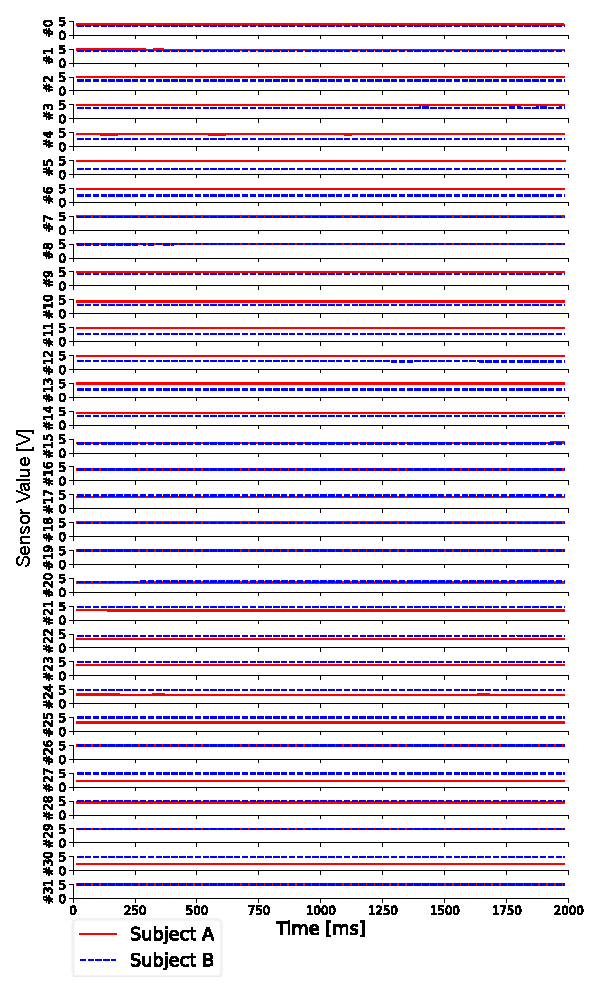
\includegraphics[width=1\linewidth]{figure/sensor_values.eps}
  \caption{\textcolor{red}{The 2-second time series values obtained from the 32 sensors for subjects A and B wearing the helmet.}}
  \label{fig:sensor_values}
\end{figure}


%4.3
\subsection{User Authentication Method}


%4.3.1
\subsubsection{Evaluation environment.}
One subject was considered the individual to be authenticated (i.e., owner) while the remaining eight subjects were considered strangers. The authentication accuracy of the owner was measured using 5-fold cross-validation, where 80\% of the owner's data (16 samples) were registered as training data and the remaining 20\% of the data (four samples) were used as test data. In addition, the authentication accuracy for strangers was measured using data from all eight strangers (160 samples). All 160 samples were tested in each fold of the cross-validation, and all nine subjects were evaluated on a rotation basis.\par

In user authentication, the false rejection rate (FRR), false acceptance rate (FAR), and equal error rate (EER) were used as indicators of authentication accuracy. The FRR is the rate at which a registered user is mistakenly considered a stranger and rejected, whereas the FAR is the rate at which a stranger is mistakenly considered a registered user and authenticated. The smaller the threshold value $\theta$ in \textcolor{red}{equation (\ref{eqn:authentication}) in section \ref{sec:authentication_decision}} is set, the stricter the authentication decision becomes, resulting in an increased FRR. In contrast, the larger the threshold value $\theta$ is set, the looser the authentication decision becomes, resulting in an increased FAR. There is thus a trade-off between the FRR and FAR, and the value at which the FRR and FAR are equal is called the EER. The EER value is commonly used as an indicator to evaluate the performance of authentication methods, and a small EER indicates better performance.


%4.3.2
\subsubsection{Results and discussion.}
The EER of each subject is presented in \tabref{tab:EER_num}. In this table, ``Average'' represents the average EER of all subjects. The FRR and FAR values for each subject by varying the thresholds from 0 to 60 by 1 are presented in \figref{fig:EER}. In this figure, ``Average'' represents the average FRR and FAR of all subjects. The EER of subjects A, E, G, and I was approximately 0.01 or lower, which signifies that the owner failed authentication less than once in 100 times and that strangers broke the authentication less than once in 100 times. An EER of 0.0097 for user authentication using ear acoustics was reported in Ref. \cite{ear_auth}; therefore, our method achieved comparable performance for four of nine subjects.\par

\begin{table}[!t]
  \centering
  \caption{Equal error rate (EER) for subjects in user authentication.}
  \begin{tabular}{c|c} \hline\hline
    Subject & EER \\ \hline
    A & 0.002 \\
    B & 0.095 \\
    C & 0.050 \\
    D & 0.055 \\
    E & 0.006 \\
    F & 0.094 \\
    G & 0.012 \\
    H & 0.050 \\
    I & 0.000 \\ \hline
    Average & 0.076 \\ \hline
  \end{tabular}
  \label{tab:EER_num}
\end{table}

\begin{figure}[!t]
  \centering
    \includegraphics[width=1\linewidth]{figure/EER.eps}
  \caption{False rejection rate (FRR) and false acceptance rate (FAR) for subjects in user authentication.}
  \label{fig:EER}
\end{figure}

The next most accurate subjects were C, D, and H, with an EER of approximately 0.05. To determine the cause of the decline in accuracy compared with subjects A, E, G, I, all collected data were compressed to the first principal component and second principal component by principal component analysis (PCA). The results of the data plotted on a two-dimensional plane are presented in \figref{fig:PCA}. The plots for subject C indicate that one sample of the data of subject C was close to the data of subject I and the variance in the first principal component was large, which would reduce the accuracy. Furthermore, the data for subjects D and H significantly overlapped with each other, which affected the accuracy of both subjects.\par

\begin{figure}[!t]
  \centering
    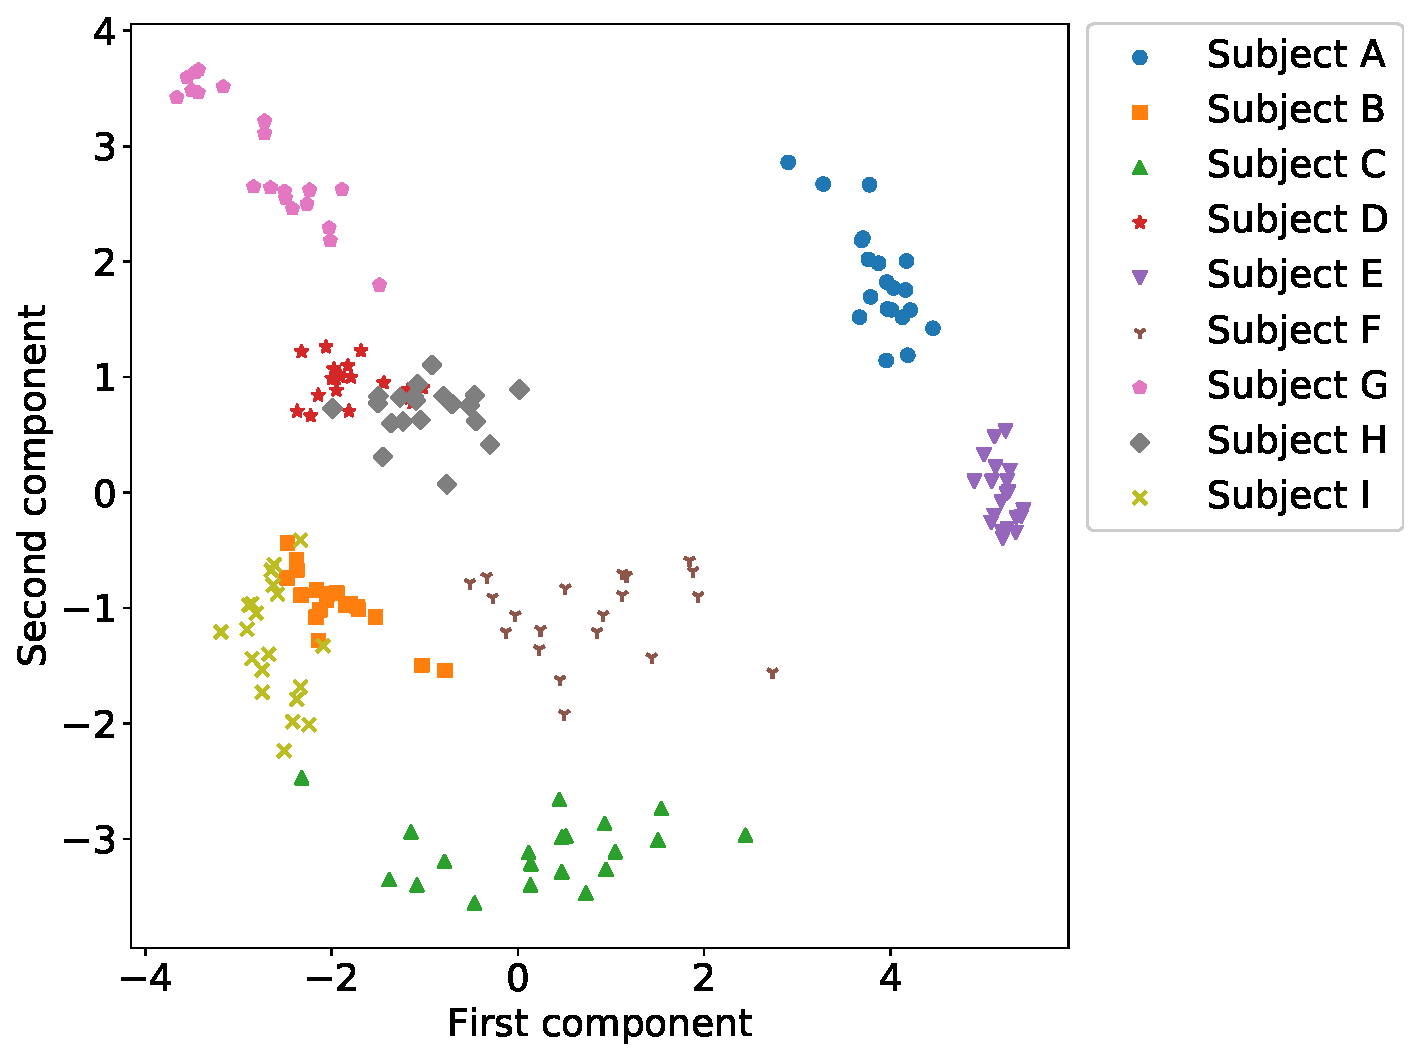
\includegraphics[width=1\linewidth]{figure/PCA.eps}
  \caption{Principal component distribution of 32-dimensional features compressed into two dimensions by principal component analysis.}
  \label{fig:PCA}
\end{figure}

The least accurate subjects were B and F, with an EER of approximately 0.095. Data for subject B was some overlap with the data of subject I. However, the EER of subject I was 0, which indicates perfect authentication. Therefore, the overlap of these data groups was likely due to the loss of data when they were compressed into two dimensions by PCA. On the other hand, subject F's data did not exhibit any overlap with other subjects' data; however, there was a large variance in both directions for the first and second principal components. Considering the effect of data compression by PCA, duplication with other subjects' data groups can be inferred in the 32-dimensional data. The accuracy for subjects B and C, who had data groups located close to subject F's data groups, may have been affected by the scattered data of subject F. In particular, the accuracy of subject B was likely to be lower than that of subject C because the two samples of subject B were located in close proximity to subject F's data group.\par

The data of subject E were located at the rightmost points. In addition, the variance was small, and the data were thus considered distinct. For subject E in \figref{fig:EER}, the FRR and FAR crossed at a threshold of approximately 60, which was greater than for the other subjects. This is because the data were quite different from the others, and the FAR did not increase by increasing the threshold.\par

\textcolor{red}{In summary, the mean EER of all subjects in user authentication was approximately 0.076. An authentication method with grip gestures using pressure sensors\cite{murao_grip} reported the average EER of 0.02. Our method is not as accurate as this method. In order to improve the accuracy, it is necessary to consider an authentication method using time series pressure data from the start of wearing the helmet to the complete of wearing.}

% In summary, the mean EER of all subjects in user authentication was approximately 0.076. It is necessary to validate with data from a larger number of subjects, as there was a difference in the EER between subjects. In addition, it is necessary to investigate a method for authentication using time series pressure data from the start of wearing the helmet to the complete of wearing.



%5
\section{Limitation}
\label{sec:limitation}
\textcolor{red}{From the results in Section \ref{sec:evaluation}, it can be seen that we were able to identify the subjects with high accuracy in the experimental environment. This section discusses the limitation of the proposed method.}


%5.1
\subsection{Restrictions on subjects and helmets}
\label{sec:subjects_and_helmets}

\textcolor{red}{In this method, the strength of the contact between the head and the helmet is obtained as the feature values using a pressure sensor. Therefore, if there is no change in the shape of the head, it can always be identified correctly regardless of age, gender, or body size. On the other hand, if the hairstyle changes, the strength of the contact between the head and the helmet will change, and the system will not be able to correctly identify the user. If the sensor mounting position is moved, the accuracy may decrease because the the feature values changes. For the same reason, it is not possible to use the same registration data for different helmets, because the feature values are affected by the size and weight of the helmet. User registration phase is required for each helmet. In the future, it is necessary to consider a calibration method based on helmet size and weight data.}


%5.2
\subsection{Helmet size adjustment}
\label{sec:helmet_size_adjustment}

\textcolor{red}{In this experiment, the helmet size was not adjusted for each subject, and all subjects used the same helmet to collect data. We think that when helmets are shared, the size is not adjusted for each user. On the other hand, if multiple sizes of helmets are given, such as S/M/L, the data with the helmet to be used must be registered. In the case of a personal helmet, the evaluation should be done by preparing a helmet that fits each wearer individually. However, only one type of helmet was used in this experiment. If the best helmet is used for each subject, the system will be able to obtain accurate data on the head shape of the registrant, and the system will not be able to obtain accurate data on the head shape of the non-registrant whose helmet size does not fit. Therefore, we think that the performance of the proposed method will be improved. In the future, we will evaluate the proposed method in these environments.}


%5.3
\subsection{Identifiable scale}
\label{sec:identifiable_scale}

\textcolor{red}{In a large construction site, approximately 1,000 workers may work together. Zhuang et al.\cite{head_shape_variations} reported that they could classify 1,169 people with 90\% accuracy using 50 data points obtained from 3D head data. Therefore, if we use a large number of pressure sensors, we may be able to classify nearly 1,000 people. The number of sensors can be increased because there is enough space between the pressure sensors in the prototype device. To find effective sensor positions, it is necessary to increase and verify the data.}


%5.4
\subsection{Comparison with common authentication methods}
\label{sec:comparison_of_performance}

\textcolor{red}{An authentication method based on individual differences in the head\cite{skull_auth} reported an EER of 6.9\%. The average EER of our method was 0.076 (7.6\%), which is roughly equivalent to the accuracy of the previous method. In the previous method, they played white noise from a bone conduction speaker attached to the side of the head, received signals using a microphone, and identified the subjects based on their characteristics. However, the helmet may be used in noisy environments such as construction sites, so this authentication method may be affected by noise. On the other hand, since our method is based on the shape of the head, it is not susceptible to noise from sound. A fingerprint authentication method using geometric features\cite{finger_geometric} reported an EER of 0.8\%. It can be seen that our method is inferior to fingerprint authentication in terms of accuracy and robustness. An authentication method based on the features of three-dimensional shapes is difficult to break through by replication, but the reproducibility of the data is low.}


%5.5
\subsection{Determination of the threshold}
\label{sec:determination_of_the_threshold}

\textcolor{red}{In an actual environment, the data of multiple users should be obtained in advance at the development stage. Then, the threshold value at which the EER is obtained can be calculated when the user's data is registered multiple times. However, the threshold value in a real environment should be determined based on the purpose of its use, just like any other biometric authentication. In the ``User authenticate when riding motorcycle'' example, vehicle theft needs to be firmly prevented. In this case, the FAR needs to be reduced, so the threshold should be determined to be small, i.e. tight.}



%6
\section{Conclusion}
\label{sec:conclusion}
In this study, we proposed a method to identify individuals based on differences in head shape, which was measured by wearing a helmet with pressure sensors. We implemented the prototype device and evaluated our proposed method. The prototype device was a commercially available full-face helmet, and we attached 32 pressure sensors inside the helmet. In the evaluation, we obtained sensor values for 2 s 20 times from nine subjects as head shape data. Using the acquired data, we evaluated the user identification accuracy to determine which user was wearing the helmet among the registrants. In addition, we evaluated the user authentication accuracy to determine whether the helmet wearer was the registrant.\par

As the accuracy was 100\% with 32 sensors in user identification, we tested how the accuracy changed by decreasing the number of sensors. The results indicated that the smallest number of sensors producing 100\% accuracy was five. The EER of four out of nine subjects was less than 0.012, and the average EER in authentication was 0.076. These results suggest that our method is effective as a user identification method. In the future, we will collect additional data and evaluate the proposed method in a real environment.



\bibliographystyle{ipsjunsrt-e}
\bibliography{references}


% \begin{biography}
% \profile{Taro Joho}{was born in 1970. He received his M.S.\ degree from
% Johoshori University in 1994.
% He joined
% the Information
% Processing Society of Japan in 1994.
% He is currently an associate professor at
% \mbox{Johoshori} University.
% His research interest is online
% publishing systems. He is a member of the IEEE and ACM\@.}
% %
% \profile{Hanako Shori}{was born in 1960. She received her M.E.\ and
% Ph.D.\ from Johoshori University in 1984 and 1987, respectively. She
% became an associate professor at Gakkai University in 1992 and a
% professor at Johoshori University in 1997. Her current research
% interest is online publishing systems. She received the Kiyasu Kinen
% award in 2010. She is a Board Member of the IPSJ and a member of the
% IEICE, IEEE-CS, and ACM\@.} 
% %
% \end{biography}
\end{document}